\documentclass[tikz]{standalone}
\usepackage{tikz}
\usepackage{fourier}
\usepackage{physics}
\usetikzlibrary{shapes.geometric}
\usetikzlibrary{calc}

\begin{document}
\begin{tikzpicture}
    \node[inner sep=0] at (0, 0) {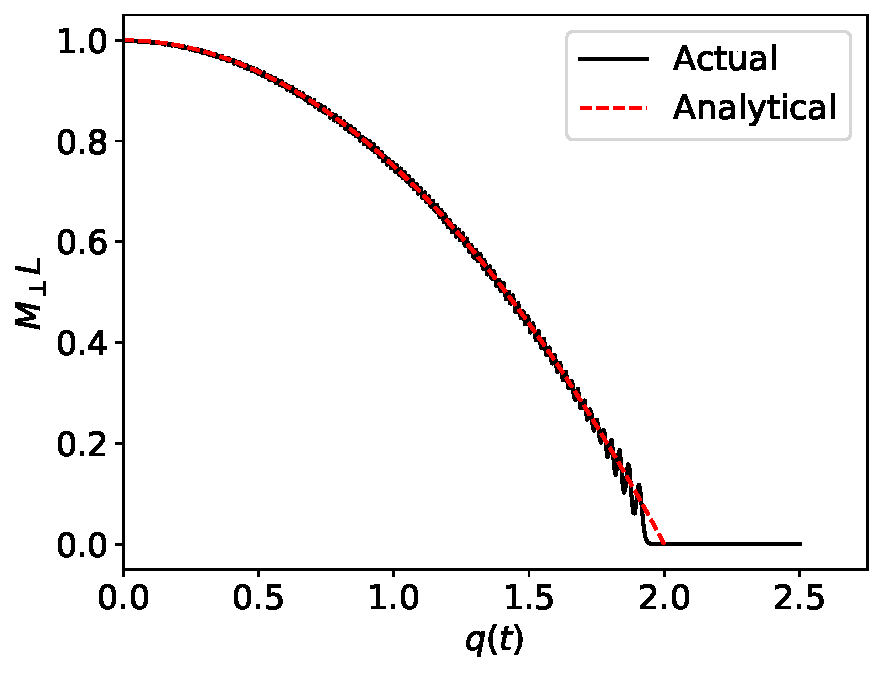
\includegraphics[scale=0.75]{../gfx/magnetisation_vs_Q.pdf}};
    \node at (0.2, -4) {\Large \(Q(t)\)};
\end{tikzpicture}
\end{document}

